\chapter{Computational Background}\label{ch:computational}

\begin{figure}[h]
    \centering
    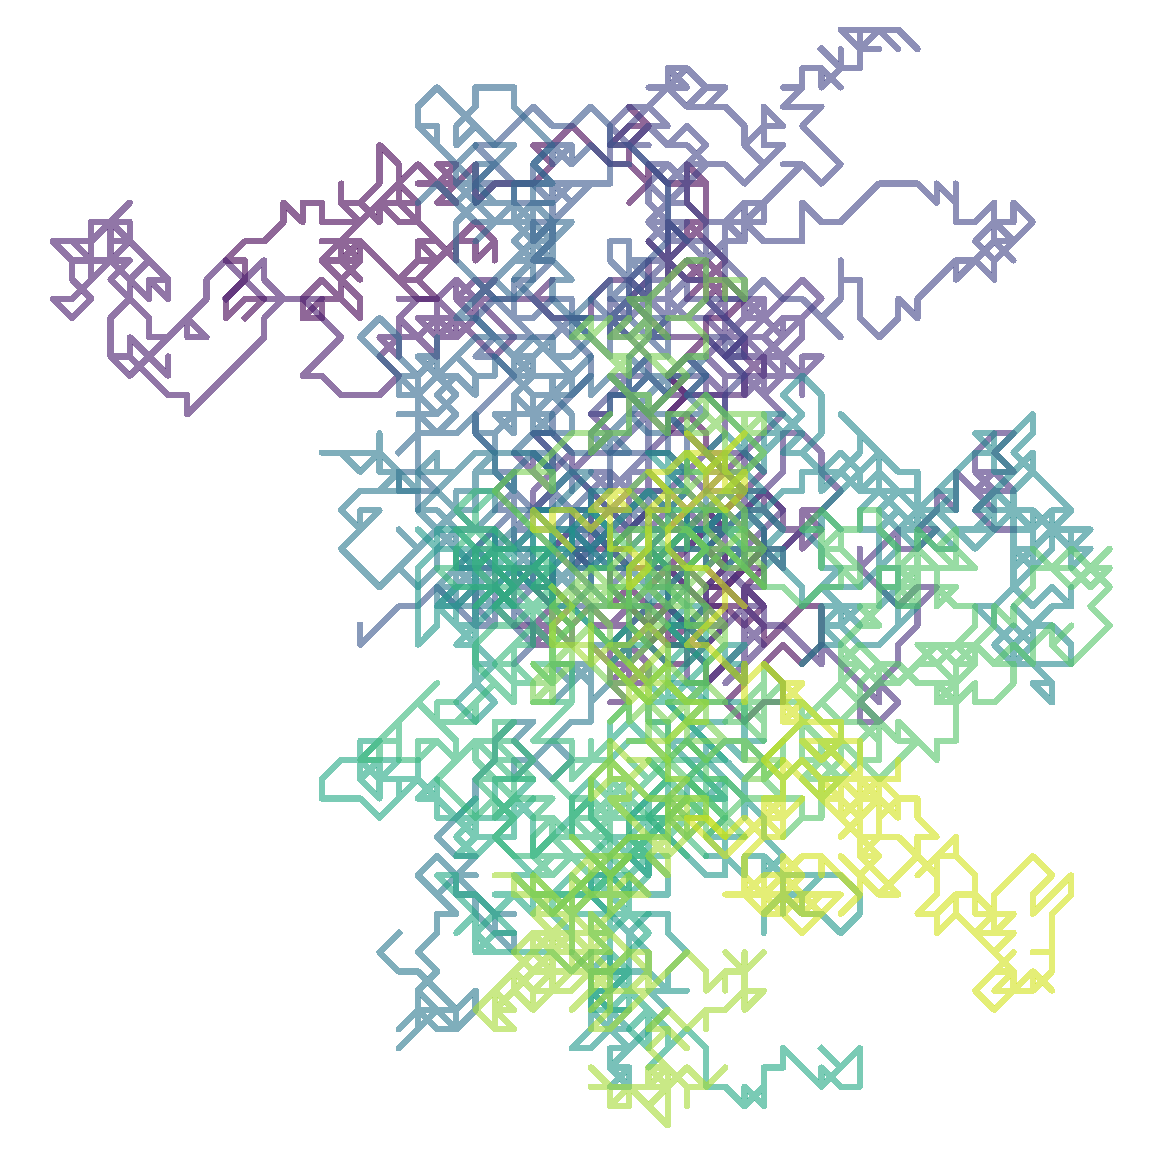
\includegraphics[width=0.8\linewidth]{Chapters/Theoretical_Background/images/random_walkers.pdf}
    \caption{Trajectory of 15 random walkers on a lattice, inspired by \cite{Nordhagen2019}.}
    \label{fig:walkers}
\end{figure}


\section{Sampling and Markov Chains}\label{sec:markov_chains}

Suppose that we wish to study a phenomenon in nature that is inherently stochastic and for which we lack prior information about its probability distribution. Then, collecting information from one single experiment is not significant. If we want to infer statistics from a set of events, we rely on sampling.

By sampling, we mean selecting a subset of a population from which to collect information. Doing so with specific statistics techniques allows us to infer information from the whole population without measuring every instance and with a good notion of how wrong the inferred values are. To eliminate unwanted bias in this collection process, it is common to conduct sample selection with some level of randomness.

In this discussion, random or stochastic variables will be denoted as $X$ and represent a function that maps a set of outcomes $\Omega=\{\text{outcome A}, \text{outcome B}\}$ to a set of numbers, for example $\{23, \pi\}$. To quote A. Eagle (2014) \cite{chancevrandomness}, one sees that a random variable is ``... neither random nor a variable''.

In the context of random variables, we will represent $P$ as the probability measure, defined in the sample space, while $p$ is its probability density function. Furthermore, we represent a conditional probability as $P(X=x | Y=y)$, that is, a probability of random variable assuming definite value $x$ given the knowledge that $Y$ has been evaluated $y$.

\subsubsection{Markov Chains}

A family of random variables indexed with a sequential notion $\{X_i\}$ is called a stochastic process. While this indexing could be discrete or continuous, in computer simulations we will work with discrete-time Markov chains. Furthermore, we disclaim that this section will compromise mathematical rigour in favour of a short and intuitive presentation of Markov chains. Therefore, some concepts such as irreducibility, ergodicity, and detailed balance will sometimes be used interchangeably.

A Markov chain is a specific type of stochastic process in which the notion of the future outcome is dependent only on the outcome of the current step, and not on the previous ones. More specifically, if the outcome of a random variable of the stochastic process is $X_{i^*} = x$, the outcome of $X_{i^* + 1}$ depends only on the value $x$, and not on any other $\{X_{j}\}_{j < i^*}$.

The way in which the Markov chain evolves is modelled
by the likelihood of a transition between two states, $t(x, y)$, where $x$ and $y$ belong to $S$, the space of all the outcomes of the stochastic variables. To correctly specify a Markov chain, we need an initial probability distribution $\pi_0$ at initial state, and the transition probabilities of the following states, meaning 
\begin{align*}
    P(X_0 = x) &= \pi_0(x), \\
    P(X_{n+1} = x_{n+1} | X_n = x_n) &= t(x_n, x_{n+1}).
\end{align*}

Note that we did not need to specify the previous states of the chain in the conditional probability, as per the definition of Markov chains. Sampling from this chain can be done by first sampling $X_0$ according to $\pi_0$, and subsequently sampling $X_n$ following $t(X_{n-1}, \cdot)$. 

It is common to associate $t(x,y)$ to elements in a transition matrix, representing the probability transition $x \to y$  of one time step. In this case, it makes sense to see $p^m = P(X_{n+m} = y | X_n = x)$ as matrix $t$ being applied in succession. Furthermore, the probability distribution guiding the outcome of the random variable $X_n$ can be written
\begin{align*}
    P(X_n = x) \equiv \pi_n(x) = \pi_0 t^n.
\end{align*}

There are several conditions that must be satisfied for our process to be a relevant Markov chain. For example, fixed a state $x$, there must be transition altogether (even if to the same state), so
\begin{align*}
    \sum_{y \in S} t(x, y) = 1.
\end{align*}

Another subtle point is that, since we study these chains for long-time evolutions, we want stochastic processes with ``nice'' asymptotic behaviour. For that to be possible, some requirements must be satisfied. First, we do not care about chains that go to subsets of the state space and never return. That would cause the isolation of the chain in a way that leads to a divergence in statistical quantities. More specifically, we say we want to study irreducible chains: chains for which any state can be reached in some finite number of steps. 

Looking at the other extreme case, we also do not want to study periodic chains, for a similar problem of lack of convergence to a stationary distribution. These conditions are usually condensed into the requirement that the Markov chain satisfies a so-called detailed balance condition, formulated as follows: $\forall x, y \in S \times S$, 
\begin{align}
    \pi(x)t(x, y) = \pi(y)t(y, x).
    \label{eq:detailed_balance}
\end{align}

That means that when the distribution has reached a steady distribution, the proportion of transitions from state $x$ to $y$ is the same as from $y$ to $x$. Given detailed balance, we can invoke two convergence theorems for finite-state Markov chains. The first one, with respect to the convergence of the distributions, and the other one with respect to the expected values of functions of the random variables. Those are the expected values we seek to sample.

First, if we have $t(x,y)$ the transition matrix of irreducible, aperiodic finite state Markov chains, $\forall x,y \in S \times S$, any initial distribution $\pi_0$ will lead to $\pi_n$ which converges to a stationary $\pi$, and we write 
 \begin{align}
     \lim_{n \to \infty} t^{n}(x, y) = \pi(y).
     \label{eq:chain_convergence1}
 \end{align}

Furthermore, for that stationary $\pi$ and considering $f(x)$ any function on the state space, for any initial $\pi_0$ it follows
\begin{align}
 P\left(\lim_{n \to \infty} \frac{1}{n}\sum_{k=1}^n f(X_k) = \sum_x f(x)\pi(x)\right) = 1.
 \label{eq:chain_convergence2}
\end{align}

This means that the expected value of $f$, which depends on the random variable, when sampled towards infinity, will tend to ever better approximate the true expected value of $f$. This theorem is crucial for Markov chain Monte Carlo, and it leads us into the topic of Monte Carlo methods.


\section{Markov Chain Monte Carlo}

\subsubsection{Monte Carlo Methods}
Monte Carlo (MC) methods are a very broad class of computational methods that use sampling to generate numerical results. These methods are used in scenarios where traditional computational approaches are impractical, making it more feasible to tackle the problem by introducing randomness and depending on the law of large numbers for approximate solutions. First seen as a ``last resort'', MC is now considered a robust approach, present extensively in scientific computing \cite{whyMC}.

Monte Carlo methods can be used to solve both probabilistic and deterministic problems. A probabilistic example would be risk assessment simulations, while a deterministic example would be calculations of intractable integrals. We will use Monte Carlo methods in two very intertwined contexts: for the evaluation of high-dimensional integrals and for sampling quantities that follow complicated or unknown probability distributions via Markov chains.

This sampling process for Monte Carlo methods is stochastic and the information obtained about the data is an inferred probability distribution with an associated random error. Despite this randomness in the estimation, the uncertainty range can be arbitrarily reduced, given the sufficient computational time, as eluded to in \eqref{eq:chain_convergence1} and \eqref{eq:chain_convergence2}.
 
To demonstrate this, let us explore the approximation of an integral using Monte Carlo sampling. Suppose that we want to compute the integral of a function $f(\mvec{x})$, over $\Omega \subset \mathbb{R}^d$, which has volume V. The naive MC approach is to sample uniformly $n$ points, $x_i$ of $\Omega$ to compute the fraction of these samples that is evaluated below $f(\Omega)$. Of course, the probability of this happening must be proportional to the magnitude of $f(x_i)$ and, consequently, to the integral value. Mathematically, this approximation boils down to
\begin{align}
    \int_\Omega f(\mvec{x})\,d\mvec{x} \approx V \frac{1}{n}\sum_{i=1}^{n} f(\displaystyle \rvx_i).
    \label{eq:mc_integration}
\end{align}

\subsubsection{A comment on random number generation}
The generation of truly random numbers in computer programmes is not feasible. What we do instead is generate apparently uncorrelated numbers with deterministic algorithms called pseudo-random number generators (PRNGs). Given a known initial state determined by a number $X_0$ which we call a seed, the algorithm can replicate a whole sequence $X_n$ of apparently random numbers. There are a myriad of PRNGs, with significant differences in terms of randomness quality, speed, cycle, and other characteristics. 

For a true uniform random variable, the generated numbers should be completely uncorrelated, and, in PRNGs, we try to avoid correlations between generated numbers as much as possible. However, since their number generation is deterministic, some level of correlation is inevitable, even if subtle.

In computer simulations, where random numbers are generated millions of times, a fast algorithm is absolutely essential. For illustration, we mention a well-known and reasonably fast algorithm: the Linear Congruential Generator (LCG). An LCG is defined by the recurrence relation
\begin{align*}
    X_{n+1} = (aX_n + c) \mod m,
\end{align*}
where the choice of $m$, $a$, and $c$ determines the specific generator and how long of a sequence of pseudo-random numbers will be before starting to repeat. The length of such a sequence is called the cycle, and modern PRNGs have cycles of around $2^{128}$ numbers.

Although PRNGs typically generate numbers uniformly between 0 and 1, there are techniques to enable these generators to produce numbers following specific, well-known distributions, such as the Gaussian distribution. Among these methods are the reverse transform method, rejection sampling, and transformation techniques such as the Box-Muller method. Ideally, when one wants to generate random samples following a specific low-dimensional distribution, these methods are excellent choices. Unfortunately, in higher dimensions, these become extremely inefficient, motivating the search for other algorithms. To illustrate this, we briefly introduce the rejection sampling method. Although we do not explicitly use it, it is a perfect bridge between Monte Carlo integration and Markov chain Monte Carlo.

\subsubsection{Rejection Sampling and Curse of Dimensionality}

\begin{figure}[h]
    \centering
    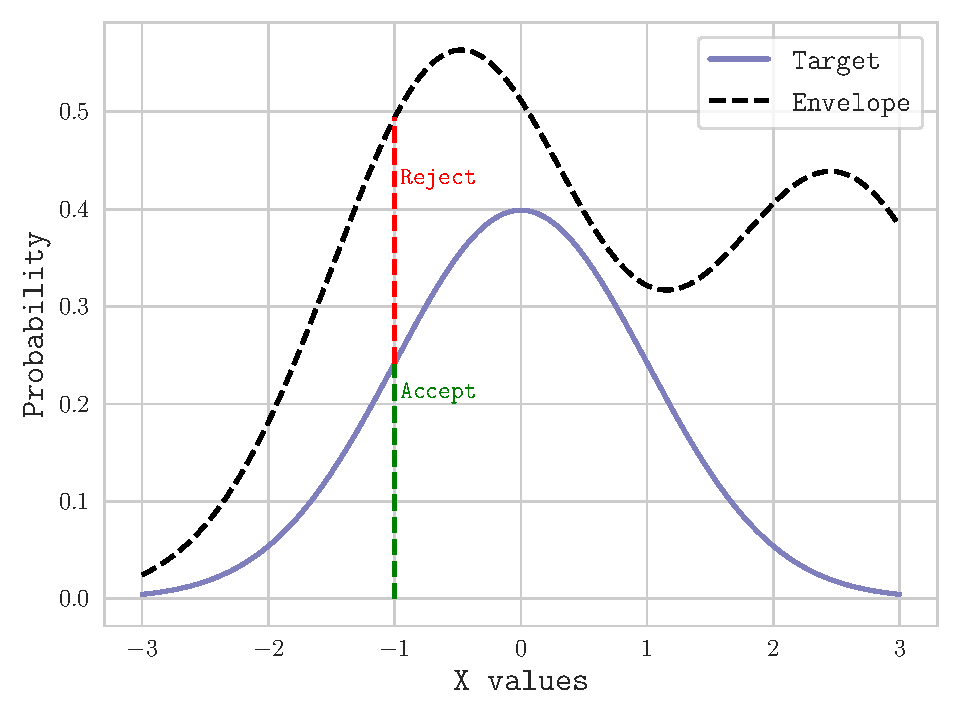
\includegraphics[width=0.6\linewidth]{Chapters/Theoretical_Background/images/rejection_sampling.pdf}
    \caption{Illustration of rejection sampling with an envelope and target distributions. Probabilities are not normalized.}
    \label{fig:rej}
\end{figure}

The idea of rejection sampling is to use a distribution from which we know how to sample, $g(x)$, to guide the sampling process and mimic the sampling of the distribution we desire, $p(x)$. This will work as long as $g$ is an envelope for $p$. More specifically, we need $p(x) < K g(x)$ for some scaling constant $K > 1$ and at any point in the function's domain. The iterative sampling process then follows three steps, which can be better understood with \figref{fig:rej}.
\begin{itemize}
    \item Sample a point $x$ from an envelope proposal distribution $g(x)$;
    \item Sample $y$ form the uniform $U(0, Kg(x))$;
    \item Accept and keep track only of samples for which $y < p(x)$.
\end{itemize}

With that, the normalised histogram that forms from the accepted samples tends to approximate the target distribution, indicating that the accepted samples indeed follow $p$. The problem with such a procedure, which is hard to see in low-dimensional examples, is that the rate of convergence for the approximation becomes slow in higher dimensions. The sampling is inefficient. In fact, the volume of rejected samples will increase at a much faster rate than that of the accepted ones, requiring a number of samples that is impractical. This is a consequence of the curse of dimensionality. 


\subsubsection{Markov Chain Monte Carlo}
To finally connect the concept of Monte Carlo integration with Markov chains, we can ask ourselves what would happen if, in \eqref{eq:mc_integration},  we sampled domain points using a general probability distribution $p$ instead of a uniform one. Recall that the expected value of a sample of $x$ following a probability distribution $p$ is denoted
\begin{align*}
    \E_{\rx\sim p}[f(X)] = \int f(x)p(x) dx,
\end{align*}
where we omit the domain for simplicity. If we compute the expected value of a function evaluated on domain points sampled following $p$ we solve a related but not exactly the same problem as the pure integral calculation of $f$. This expectation value can be approximated by the average of the samples,
\begin{align*}
    \E_{\rx\sim p}[f(\rx)] \approx \hat{\E}_{\rx\sim p}[f(\rx)] = \frac{1}{n}\sum_{i}^{n}f(x_i).
\end{align*}

As the number of samples $n$ increases, under the law of large numbers for Markov chains, this approximation will improve arbitrarily. Still, the question of how to generate samples from $p$ with Markov chains remains. As discussed in \secref{sec:markov_chains}, we require a Markov chain for which the stationary distribution is the one we want to sample from. In fact, there are different possible ways to do that, with maybe the two most common being the Metropolis and Gibbs algorithms. 

\subsection{Metropolis Algorithm }\label{sec:metropolis}

\begin{figure}[h]
    \centering
    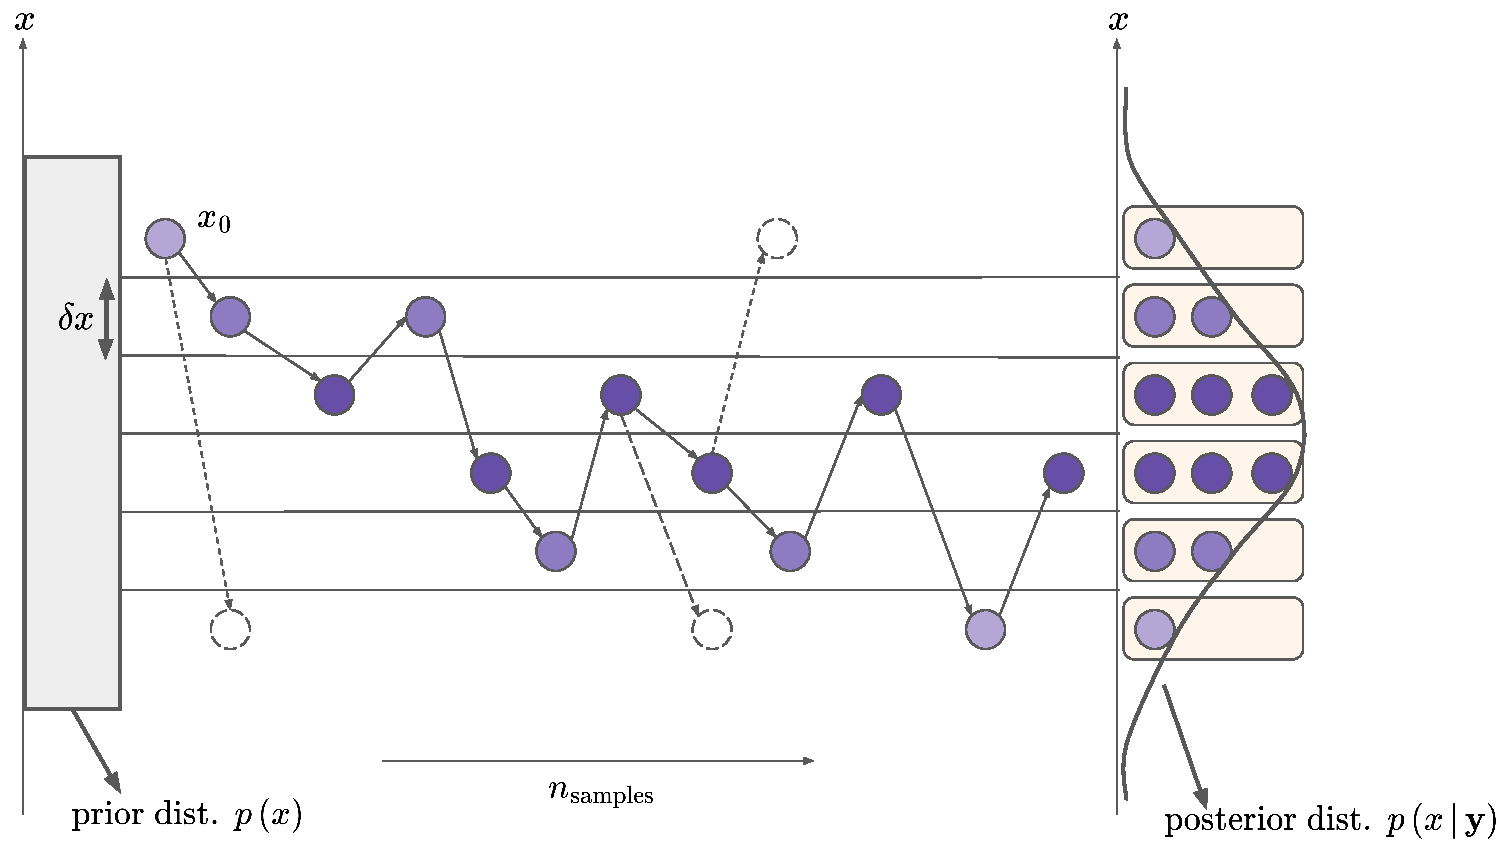
\includegraphics[width=0.8\linewidth]{Chapters/Theoretical_Background/images/metropolis.pdf}
    \caption{Illustration of using a prior distribution sampling to obtain samples from a posterior distribution by accepting and rejecting moves from an initial position $x_0$. Adapted from Lee et al., 2015 \cite{lee2015metamodel}}
    \label{fig:sampling_metropolis}
\end{figure}

Initially described in \cite{metropolisEquationStateCalculations1953}, the Metropolis algorithm serves as one method to generate a Markov chain to sample from, aiming to achieve a steady distribution that matches the target distribution. So far, we have not addressed how to get the correct transition probabilities $t(x, y)$ required from \eqref{eq:chain_convergence1}. The idea of Metropolis algorithm is to model a transition in state space via two independent probabilities. First, the transition state $y$ must be available, modelled by a proposal distribution $g(x,y)$. Moreover, there is a probability that $y$ is accepted $a(x,y)$ from the current state $x$. The fact that these are assumed independent means we can rewrite the detailed balance condition of \eqref{eq:detailed_balance} as
\begin{align*}
    \pi(x)a(x, y)g(x,y) = \pi(y)a(y, x)g(y,x),
\end{align*}
or, rearanging, 
\begin{align}
    \frac{a(x, y)}{a(y, x)} = \frac{\pi(y)}{\pi(x)}\frac{g(y,x)}{g(x,y)}.
    \label{eq:metropolis-hastrings-acceptance1}
\end{align}

Note that $g$ is something that we control and could be, for example, a normal distribution centred around the current state. Furthermore, it plays a similar role to the envelope distribution in rejection sampling. Satisfying \eqref{eq:metropolis-hastrings-acceptance1} above is equivalent to having an acceptance rule of
\begin{align}
    a(x, y) = \min\left(1, \frac{\pi(y)}{\pi(x)}\frac{g(y,x)}{g(x,y)}\right).
    \label{eq:metropolis-hastrings-acceptance2}
\end{align}

In other words, if we use such an acceptance rule with a proposal distribution that we control, we are still satisfying detailed balance. In this case, the sampled values will converge to the sampled values under the desired stationary probabilities. If we use a symmetric proposal distribution $g$ such as a normal distribution, \eqref{eq:metropolis-hastrings-acceptance2} further simplifies, given that the fraction of proposed probabilities will be one. Under this simplification, the Metropolis–Hastings algorithm is simply called Metropolis, but more often than not the names are used interchangeably.

A final comment on the Metropolis-Hastings algorithm is that, due to the fraction between $\pi(y)$ and $\pi(x)$, it allows us to sample quantities from $\pi(y)$ with any proportional probability distribution $f(x) \propto \pi(x)$. 

\secref{sec:VMC} includes an algorithmic recipe with algorithm box \ref{algo:general_update_rule}, although fitted to our variational Monte Carlo framework. In addition, \figref{fig:sampling_metropolis} illustrates the general idea of proposing steps from an initial state $x_0$ and accepting or rejecting them to generate a posterior distribution. 

\begin{JTD}
This last comment about allowing for a function $f \propto \pi$ can seem irrelevant but allows us to sample from distributions for which we lack knowledge of partition functions. In our case, it allows us to use an unnormalized ansatz in variational Monte Carlo. 
\end{JTD}

\section{Variational Monte Carlo}\label{sec:VMC}
As discussed in \secref{sec:choice_of_systems}, we are deeply interested in solving the Hamiltonian eigenvalue problem. More specifically, we are focused on the smallest eigenvalue and its eigenstate. We now see a way to approach this problem via Markov chain Monte Carlo, avoiding explicitly solving the Schrödinger equation.

By the variational principle, discussed in \secref{sec:var_principle}, any trial wave function yields and expectation value for the energy that is bounded from below by the true ground-state energy of the system. With that in mind, variational Monte Carlo (VMC) is a method that iteratively samples energy values from a parameterised trial wave function $\ket{\Psi_T(\mvec{\theta}) }$ and updates its parameters $\mvec{\theta}$ to drive the sampled energies to a minimum. VMC is heavily biased by the functional choice for the trial function, and finding a good initial guess can be extremely difficult. It is therefore an approximate method with potentially large error bars. 

Despite these challenges, VMC remains easy to implement in comparison to other more precise methods, such as diffusion Monte Carlo, while also avoiding the infamous sign problem \cite{Pan_2024}. The idea behind VMC is to note that, by using a trial wave function $\Psi_T$, one can express the expected value for any observable $O$ on a complete basis $\{\ket{\mvec{\alpha}}\}$ as 
\begin{align}
    \frac{\langle\Psi_T |\hat{O}|\Psi_T\rangle}{\langle\Psi_T |\Psi_T\rangle} &= \sum_{\mvec{\alpha}, \mvec{\beta}}\frac{\langle\Psi_T |\mvec{\alpha}\rangle\langle \mvec{\alpha} | \hat{O}|\mvec{\beta}\rangle \langle \mvec{\beta} |\Psi_T\rangle}{\langle\Psi_T |\Psi_T\rangle}\\
    &=\sum_{\mvec{\alpha}} \frac{\langle\Psi_T |\mvec{\alpha}\rangle\langle \mvec{\alpha} |\Psi_T\rangle}{\langle\Psi_T |\Psi_T\rangle}\sum_{\mvec{\beta}}  \langle \mvec{\alpha} | \hat{O}|\mvec{\beta}\rangle  \frac{ \langle \mvec{\beta} |\Psi_T\rangle}{\langle\Psi_T |\mvec{\alpha} \rangle}\\
    &=\sum_{\mvec{\alpha}}P(\mvec{\alpha})\sum_{\mvec{\beta}}O_{L}(\mvec{\beta}).
    \label{eq:exp}
\end{align}

The first term in the summation represents the normalised probability of the state $P(\mvec{\alpha})$, while the second term can be interpreted as a local operator estimator $O_L$. This allows us to approximate the expectation value on the left-hand side of \eqref{eq:exp} as the average of sampled values of the observable associated with the local operator. To better illustrate this, let us express the trial wave function as $\Psi_{\mvec{\theta}}(\mathbf{R})$ and deal with the Hamiltonian operator. This representation indicates a wave function parameterised by $\mvec{\theta}$ with $\mathbf{R}$ a collective variable of all positions of a multi-particle system. In this case, the VMC energy follows
\begin{equation}
    E(\mvec{\theta}) = \frac{\langle \Psi_{\mvec{\theta}}(\mathbf{R}) | \hat{H} | \Psi_{\mvec{\theta}}(\mathbf{R}) \rangle}{\langle \Psi_{\mvec{\theta}}(\mathbf{R}) | \Psi_{\mvec{\theta}}(\mathbf{R}) \rangle} =  \int E_L(\mathbf{R}) p(\mathbf{R}, \mvec{\theta}) \, d\mathbf{R} = \langle E_L \rangle_{\mathbf{R} \sim p(\cdot, \mvec{\theta})},
    \label{eq:vmc_energy_integral}
\end{equation}
where we have introduced the concept of a local energy $E_L$,
\begin{equation}
    E_L = \frac{\hat{H} \Psi_{\mvec{\theta}}(\mathbf{R})}{\Psi_{\mvec{\theta}}(\mathbf{R})},
    \label{eq:local_energy}
\end{equation}
and the probability density function $p_{\mvec{\theta}}(\mathbf{R})$,
\begin{equation}
p_{\mvec{\theta}}(\mathbf{R}) = \frac{|\Psi_{\mvec{\theta}}(\mathbf{R})|^2}{\int |\Psi_{\mvec{\theta}}(\mathbf{R})|^2 \, d\mathbf{R}}.
\label{eq:probability_density}
\end{equation}



This allows us to use Markov chain Monte Carlo to approximate the high-dimensional integral in \eqref{eq:vmc_energy_integral}:
\begin{equation}
\int E_L(\mathbf{R}) p_{\mvec{\theta}}(\mathbf{R}) \, d\mathbf{R} \approx \frac{1}{n} \sum_{\mathbf{R} \in \mathbf{R}_n \sim p_{\mvec{\theta}}(\cdot)} E_L(\mathbf{R}), 
\label{eq:mc_integration2}
\end{equation}
where $n$ denotes the number of samples $\mathbf{R}_n$ in a Markov chain framework. To see why this approximation is necessary, let us disregard spin degrees of freedom and try to compute the integral
\begin{align*}
    \langle H \rangle = \frac{\int dR_1 dR_2 \ldots dR_N \psi^* H \psi }{\int dR_1 dR_2 \ldots dR_N \psi^* \psi}.
\end{align*}

As detailed in \cite{hjorth-jensen2021}, evaluating this integral via Gaussian quadrature with 10 particles and 10 mesh points for each degree of freedom would take around $10^{18}$ seconds, or ten billion years. This calculation considers $10^{30}$ floating point operations in three dimensions, assuming that the calculations are performed on an ideal computer, which is totally impractical.

For an illustration on how to proceed with the calculation of the local energy of \eqref{eq:local_energy}, we can break down the Hamiltonian in terms of kinetic and potential energy. The potential term will depend on the system (external potential trap and particle particle interaction), but the local kinetic term can be written,
\begin{align*}
    \hat{K} = -\frac{1}{2}\frac{\mathbf{\nabla}^{2} \Psi_{\mvec{\theta}}}{\Psi_{\mvec{\theta}}}.
\end{align*}

For stability reasons, it is common, when dealing with VMC, to work with the wave function in the logarithmic domain \cite{sorellabook}. This approach helps especially with convergence stability, as the trial function can assume very small or very large values. The sign of the wavefunction must be kept, of course, if one wishes to retrieve the wavefunction expression and not just the probability distribution. In this case, the kinetic term follows
\begin{equation*}
    \hat{K} = -\frac{1}{2} \sum_{i=1}^N \left[ \left(\frac{\partial \ln\left|\Psi_{\mvec{\theta}}(\mathbf{R})\right|}{\partial R_i}\right)^2 + \frac{\partial^2 \ln\left|\Psi_{\mvec{\theta}}(\mathbf{R})\right|}{\partial R_i^2} \right],
\end{equation*} 
with $N$ the number of particles and $R_i$ refering to the vector coordinates of particle $i$. The derivation of this expression is available in Appendix \ref{appendix:vmc}.

The minimisation of the expectation value for the local energy can be achieved using a gradient descent optimisation approach, which will be further detailed in \secref{sec:Gradient-based optimisation}. In its simplest form, the iterative update of parameters can be represented as
\begin{equation}
    \theta_{(t+1)} = \mvec{\theta}_{(t)} - \nabla_{\mvec{\theta}} E(\mvec{\theta}),
\end{equation}
with $t$ the iteration index. A caveat here is that we are taking a derivative of the expectation value, which follows, dropping the $T$ subscript for simplicity:
\begin{align*}
    \nabla_{\mvec{\theta}} E(\mvec{\theta})= 
\frac{\int d\mathbf{R}\, (\nabla_{\mvec{\theta}}\Psi^*) H \Psi + \Psi^* H(\nabla_{\mvec{\theta}}\Psi)}{\int d\mathbf{R}\, \Psi^* \Psi }
- \frac{\left(\int d\mathbf{R}\, \Psi^* H \Psi\right) \nabla_{\mvec{\theta}} \left(\int d\mathbf{R}\, \Psi^* \Psi \right)}{\left(\int d\mathbf{R}\, \Psi^* \Psi \right)^2}.\\
\end{align*}
If we let $\mathcal{N} = \int d\mathbf{R}\, \Psi^* \Psi $ for simplicity and considering the wavefunction assumes only real values, it follows
\begin{align*}
    \nabla_{\mvec{\theta}} \mathcal{N} = 2 \int d\mathbf{R}\, \Psi \nabla_{\mvec{\theta}}\Psi 
\end{align*}
and
\begin{align*}
\nabla_{\mvec{\theta}} E(\mvec{\theta}) &= \int \frac{d\mathbf{R}\, (\nabla_{\mvec{\theta}}\Psi) H \Psi + \Psi H(\nabla_{\mvec{\theta}}\Psi)}{\mathcal{N} }
- 2\left\langle E_L\right\rangle\left\langle\Psi^{-1}\nabla_{\mvec{\theta}}\Psi\right\rangle\\
&=2\left(\left\langle E_L \cdot\Psi^{-1}\nabla_{\mvec{\theta}}\Psi\right\rangle-\left\langle E_L\right\rangle\left\langle\Psi^{-1}\nabla_{\mvec{\theta}}\Psi\right\rangle\right),\\
\end{align*}
which is also equivalent to, and more often seen as 
\begin{equation}
    \nabla_{\mvec{\theta}} E(\mvec{\theta})=2 \mathbb{E}_{\mathbf{R}\sim |\Psi_{\mvec{\theta}}|^2}\left[ \left(E_L
- E(\mvec{\theta})\right)\nabla_{\mvec{\theta}}\log \left|\Psi_{\mvec{\theta}} (\mathbf{R})\right|\right].
\label{eq:grad_el_vmc2}
\end{equation}

The real-valued wave function assumption in this derivation is reasonable in sight of our computational implementation: We will be dealing only with stationary states and bounded systems.

\subsection{Metropolis Algorithm and VMC}

With this rewriting, we move the difficulty of the problem from a high-dimensional integral to sampling from a distribution over the position space $\mathbb{R}^{Nd}$, where $N$ is the number of particles and $d$ the number of dimensions of the system. Then, a sequential Monte Carlo Markov chain proposal of steps is denoted $\Vec{R}^{(i)} \to \Vec{R}^{(i+1)}$ so that it depends only on the previous state at position $\Vec{R}^{(i)}$. Whether the new point $\Vec{R}^{(i+1)}$ should be accepted is evaluated according to an acceptance rule, such as \eqref{eq:metropolis-hastrings-acceptance2} for the Metropolis scheme. 

Given that $\Vec{R}^{(i+1)}$ represents the coordinates of all particles,  we propose new positions by moving either all particles at the same time or one at a time. Both Metropolis and the (to be discussed) Langevin Metropolis-Hastings require some proposal rule, which we write as $\mvec{\mu} = \mvec{\mu}(\mvec{\sigma}_1, \mvec{\tau}_1) \in \mathbb{R}^d$, where $\mvec{\sigma}_1$ are system-dependent parameters (such as $\Vec{R}, \Psi_T(\Vec{R})$) and $\mvec{\tau}_1$ are method-specific parameters. In addition, we define a metric $\nu = \nu(\mvec{\sigma}_2, \mvec{\tau}_2)$ used in the evaluation for the acceptance or rejection of the proposed points.

In the Metropolis algorithm, $\nu$ is compared to a random number drawn from a continuous uniform distribution $r \sim U_c(0,1)$. Should $\nu$ be larger than this number, the step is accepted. Otherwise, the configuration $\Vec{R}$ remains the same. There is also a need to initialise the particle positions, which greatly affects the convergence of the sampling. We will note this by the function $\mvec{\lambda}$, based on drawing positions following a probability distribution. In case we choose to move one particle at a time, the general movement of $\mvec{R}$ in the state space $\mathcal{S}$ can be seen in Algorithm \ref{algo:general_update_rule}. To better see how this extends in the whole context of variational parameter training, we refer to the Algorithm \ref{algo:nqs_update_rule}.
\begin{algorithm}[H]
    \begin{algorithmic}
            \STATE Initialize all particle positions $\Vec{R}^{(1)} \leftarrow \mvec{\lambda}$        
            \FOR{$i = 1, 2, \ldots, n$}
                \STATE Draw a random particle index $p \sim U_d[1,N]$ 
                \STATE Calculate new particle position $\Vec{R}'_p \leftarrow \Vec{R}^{(i)}_p + \mvec{\mu}$
                \STATE Calculate metric $w \leftarrow \nu(\Vec{R}', \Vec{R}^{(i)})$  %Assign I to I + f(x)
                \STATE Draw uniform number $r \sim U_c(0,1) $ 
                \IF{ $w \geq r $ }
                    \STATE Accept new position: $\Vec{R}^{(i+1)}_p \leftarrow \Vec{R}^{(i)}_p$ 
                \ENDIF
            \ENDFOR
    \end{algorithmic}
    \caption{Procedure to determine $n$ configurations in $\mathcal{S}$. $U_c$ and $U_d$ are continuous and discrete uniform probability distributions respectively. Here, we move one particle at a time.}
    \label{algo:general_update_rule}
\end{algorithm}

In the Metropolis algorithm, the normalisation constant of the probability density function in \eqref{eq:probability_density} will cancel when calculating the acceptance rule. More specifically, for the trial wave function of the quantum mechanical system of interest, the ratio of the trial step $\Vec{R} \to \Vec{R}'$ follows
\begin{align}
    \nu_{M}(\Vec{R}, \Vec{R}') = \frac{p(\Vec{R}')}{p(\Vec{R})} = \frac{|\Psi_T (\Vec{R}')|^2}{|\Psi_T(\Vec{R})|^2},
    \label{eq:met:metric_metropolis}
\end{align}
which leads to the acceptance rule 
\begin{align}
    a(\Vec{R}, \Vec{R}') &= \min\left(1, \nu_{M}(\Vec{R}, \Vec{R}')\right).
    \label{eq:acceptance_metro_def}
\end{align}

If a proposed step moves towards a higher probability density, $\nu_{M} > 1$, and we always accept the step. In addition, to adequately sample from the probability distribution, some steps towards lower density regions must also be accepted. To test whether this should be the case, we also compare $\nu_M$ with $r \sim U_c (0,1)$ (as can be seen in Algorithm \ref{algo:general_update_rule}). If each particle is allowed to move a step length of $\delta$ in each dimension for each iteration, using a continuous uniform distribution, the proposal rule can be written as
\begin{align}
    \mvec{\mu}(\delta) = \sum_{i=1}^{D} d_i \delta \hat{e}_{x_{i}}, \hspace{20px} d_i \sim U_c (-1, 1), \label{eq:met:update_rule_metropolis}
\end{align}
where $\hat{e}_{x_{i}}$ are single particle unit vectors. If $\delta$ is too small, only small changes of $\Vec{R}$ will be allowed between iterations, and the probability density ratio \eqref{eq:met:metric_metropolis} will often be close to one, in which case $\nu_{M} > r$ will be true for almost every step and almost every proposal will be accepted. Too high of an acceptance rate results in sample means that slowly converge to the population mean. On the other hand, if $\delta$ is too large, the proposed step $\Vec{R}'$ is likely to land in a low-density region of $p$, with most steps being rejected, little movement in $\mathcal{S}$ and many repeated samples. 

Hence, it is crucial to identify a value of $\delta$ that ensures a balanced ratio of accepted to rejected steps. This proportion, commonly known as the acceptance rate $A_r$, is generally associated with reliable results when it is approximately $0.5$ \cite{gelmanWeakConvergenceOptimal1997}.

The steps proposed by the Metropolis algorithm are in some sense naive since the proposal step $\Vec{R}'$ uses no information on the probability distribution, but only on the probability at individual points by evaluating $\nu_M$. This, once more, can lead to inefficient sampling in high-dimensional spaces and motivates the Langevin Metropolis importance sampling, to be introduced in \secref{sec:langevin_imporance}.

\section{Diffusion Monte Carlo}

Diffusion Monte Carlo (DMC) is a well-established method for employing Monte Carlo sampling and diffusion theory to computationally determine the ground-state energies in quantum systems. Although we do not use the method directly, we discuss it for two reasons. First, it is recognised for providing potentially exact results, which we use to benchmark our calculations. Moreover, DMC has been shown to require an importance sampling approach to the Metropolis algorithm \cite{kalos1974helium}. This approach, which guides the sampling distribution of the proposal steps, is also used by us in our VMC calculations. Our DMC discussion is conceptual, and a more in-depth treatment can be found in \cite{Apaja2018qmc, kosztin1996introduction}

The DMC method is motivated by looking at the time-dependent Schrödinger equation of \eqref{eq:sol_tdse} under imaginary time evolution. This means that we replace $it \to \tau$, and the solution described on an enumerable eigenbasis $\ket{\phi_i}$, ordered according to the ascending order of eigenvalues can be written
\begin{align*}
\ket{\Psi(\tau)} &= e^{-\hat{H}\tau}\ket{\Psi(0)} \\
                &= \sum_i e^{-E_i\tau} c_i\ket{\phi_i} = c_0e^{-E_0\tau}\left[\sum_i \frac{c_i}{c_0}e^{-(E_i - E_0)\tau}\ket{\phi_i}\right].
\end{align*}

This can be understood as an operator $\exp({-\hat{H}\tau})$ that acts so that other states decay exponentially to the ground-state. The closer $E_i$ is to $E_0$, the slower the decay rate. In practice, this time evolution is often unstable, and it is standard to shift the energy scale towards a trial value $E_T$, for example the energy of the non-interacting ground-state problem. Then, in the limit of long time evolution, the excited parts of the general state get projected to the ground-state, either by decaying, if $E_i - E_T > 0 $ or by amplification, in case $E_L- E_T < 0$:
\begin{align*}
\ket{\Psi(\tau \to \infty)} \to c_0 e^{-E_0\tau} \ket{\phi_0}.    
\end{align*}

Under this lens, DMC models the evolution in imaginary time as a generalised diffusion process, where energy terms act as either sources or sinks. Initially conceptualised by E. Fermi in the 1940s, this scenario is described through random walkers experiencing birth-or-death processes. 

The operator responsible for the diffusion evolution, which is now shifted by $E_T$ is the Greens's function,
\begin{equation*}
    \hat{G}(\tau) = e^{-(\hat{H} - E_T)\tau}.
\end{equation*}

After appropriate basis transformations necessary for us to solve the problem computationally, it is possible to write the Green's function in such a representation that yields 
\begin{equation*}
    \Psi(\mathbf{R}, t + \tau) = \int G(\mathbf{R},\mathbf{R}',\tau) \Psi(\mathbf{R}', t + \tau) d\mathbf{R}'.
\end{equation*}

Furthermore, under what is called the short-time approximation for the Green's function, one is able to approximate $G$ as a product of a diffusion part, $G_d$, and a branching part $G_b$, with $G_d$ attributed to the kinectic energy and $G_b$ to the potential energy.
\begin{equation}
    G(\mathbf{R},\mathbf{R}',\tau) \approx G_d(\mathbf{R},\mathbf{R}',\tau)G_b(\mathbf{R},\mathbf{R}',\tau)
\end{equation}

We now provide a brief description of how the rest of a naive DMC algorithm would be carried out. For each iteration, the branching part $G_b$ is used to evaluate whether walkers should be created or destroyed from the sampling procedure. Then, the walkers positions are allowed to move following the diffusion due to $G_d$. The specifics of the branching process and subsequent data collection are not covered in this discussion. Nevertheless, we explore further the diffusion process as it provides inspiration for our VMC implementation.

The diffusion Green's function must satisfy the diffusion equation:
\begin{equation}
    \frac{\partial G_d(\mathbf{R},\mathbf{R}',\tau)}{\partial_\tau} = -D \nabla^2_\mathbf{R}G_d(\mathbf{R},\mathbf{R}',\tau),
\end{equation}
in which case the solution is 
\begin{equation}
    G_d(\mathbf{R}',\mathbf{R},\Delta t) = \frac{\exp{\left(-\frac{(\mathbf{R}'-\mathbf{R})^2}{4D\Delta t}\right)}}{(4\pi D\Delta t)^{3N/2}}, 
\end{equation}
with D a diffusion constant and $\Delta t$ a free parameter time step. In the quantum mechanical case, $D = \hbar^2/2m$ or, in natural units, simply $D = 1/2$. If no importance sampling algorithm is used, such distribution can be sampled by making walkers move similarly to standard metropolis algorithm with a proposal
\begin{align*}
    \mathbf{R}' = \mathbf{R} + \mvec{\eta}\sqrt{2D\Delta t},
\end{align*}
with $\mvec{\eta}$ such that for each particle, $\eta$ is a d-dimensional Gaussian. Then, the acceptance criteria follows
\begin{align*}
    a(\Vec{R}, \Vec{R}') &= \min\left(1, \frac{G(\mathbf{R}',\mathbf{R}, \Delta t)}{G(\mathbf{R}, \mathbf{R}', \Delta t)}\nu_M\right),
\end{align*}
with $\nu_M$ the metropolis metric. However, as already mentioned, DMC requires a more guided sampling process, which we introduce now. 

\subsection{Langevin Metropolis Importance Sampling}\label{sec:langevin_imporance}
Often in quantum-mechanical simulations, the probability distribution to be inferred from sampling can be somewhat localised. Then, a significant portion of the stochastic integration steps gets wasted in regions that are not representative of the target distribution. More critically, unguided Monte Carlo sampling leads DMC walkers towards regions of infinite potential and unstable results.

The Langevin Metropolis importance sampling method aims at guiding the acceptance probability to the target distribution of the trial wave function. This is done by introducing a quantum force or drift force, as explained in depth in \cite{chin1990langevinimportance}. Under the action of a drift force, $\mathbf{F}$, the evolution of a probability distribution $P(\mathbf{R}, t)$ can be modelled by the Fokker-Planck equation:
\begin{equation}
\frac{\partial P(\mathbf{R}, t)}{\partial t} = D\nabla\left[(\nabla - \mathbf{F}(\mathbf{R}))P(\mathbf{R}, t)\right].
\label{eq:fokker_plank}
\end{equation}
The relation between $\mathbf{F}$ and $P$ can be further investigated under some assumptions. It can be shown \cite{Fleisher2018} that since the force must act in the orthogonal direction of the diffusion, and given that in the stationary state, the left-hand side of \eqref{eq:fokker_plank} must be zero, the quantum force can be expressed as $\mathbf{F} = P^{-1}\nabla P$. In this case, for a particle $k$ at position $\mathbf{R}_k$,
\begin{equation*}
    \mathbf{F}(\mathbf{R}_k) = \frac{2\nabla\Psi(\mathbf{R}_k)}{\Psi(\mathbf{R}_k)}.
\end{equation*}

Invoking now the Langevin equation \cite{van1992stochastic}, which tells us how a stochastic variable can evolve under the time evolution of the distribution, a proposal $\mathbf{R}' = \mathbf{R} + \mvec{\mu} $ is given by 
\begin{align}
    \mvec{\mu}(\Vec{R}, \Delta t) &= D \mathbf{F}(\Vec{R})\Delta t +  \xi \sqrt{\Delta t} \label{eq:met:update_rule_metropolis_hastings},
\end{align}
with $\xi$ following a $d$-dimensional Gaussian distribution and $\Delta t$ follows the similar role as the step-length in regular Metropolis. The importance sampling algorithm then expresses the distribution $g$ in the acceptance rule of \eqref{eq:metropolis-hastrings-acceptance2} as the solution for the Fokker-Planck equation, which is the Green's function
\begin{equation}
    G_d(\mathbf{R}',\mathbf{R},\Delta t) = \frac{\exp{\left(-\frac{(\mathbf{R}'-\mathbf{R}-D\Delta t \mathbf{F}(\mathbf{R}))^2}{4D\Delta t}\right)}}{(4\pi D\Delta t)^{3N/2}}, \label{eq:met:metric_metropolis_hastings}
\end{equation}
which corresponds precisely to the diffusion component of the Green's function in the DMC context, $G_d$, now incorporating a drift term. If we are using a VMC algorithm instead of DMC, there is by definition no branching part of the general Green's function. In that case, we can express the modified acceptance criteria of this method as 
\begin{align}
    a(\Vec{R}, \Vec{R}') &= \min\left(1, \nu_{LMH}(\Vec{R}, \Vec{R}')\right), \notag\\
    \nu_{LMH}&=\frac{G_d(\mathbf{R}',\mathbf{R}, \Delta t)}{G_d(\mathbf{R}, \mathbf{R}', \Delta t)}\nu_M.
    \label{eq:acceptance_langevin_metro_def}
\end{align}

In words, the importance sampling guidance works by adjusting the acceptance probability such that the metric of \eqref{eq:met:metric_metropolis} is multiplied by the fraction of two Green's functions that model the transition probability between state $\mathbf{R}' \to \mathbf{R}$ of a probability distribution evolving due to a diffusion and a quantum force. In contrast to Metropolis, this algorithm adds, both in \eqref{eq:met:metric_metropolis_hastings} and \eqref{eq:met:update_rule_metropolis_hastings}, physical information about the trial wave function, indicating at least in theory a more robust method.

\subsubsection{A comment on DMC}

One of the advantages of DMC over VMC is that, in VMC, occasional excited states can contribute to the minimised energy via local minima, whereas in DMC calculations, excited states exponentially decay to the ground-state in the imaginary time evolution.

Despite being extremely precise, DMC also presents a couple of drawbacks. First, there is the constant problem of computational cost. For bosonic systems, DMC scales polynomially with the system size, but for fermionic systems, the scaling is exponential. Furthermore, and perhaps more important, is the fermionic sign problem: DMC can only be performed assuming wave functions that are positive at any evaluated point. Although techniques are used to circumvent this, such as the fixed node approximation \cite{anderson1975random}, they all bias the samples in some way.
